\section{Геометрические свойства модели Ising-ISAW с точки зрения числа соседей в узлах}

\subsection{Введение}

В данном разделе мы изучаем такое геометрическое свойство модели, как доли узлов с фиксированным числов соседей. У каждого узла можно определить число соседей или количество близких связей на смежных ячейках исследуемой решётки. Рассмотрим пример конформации на квадратной решётке на рисунке \ref{fig:example_bulk}. Чёрные точки соответствуют узлам с 2-мя соседями, а последовательность таких узлов подряд в конформации можно интерпретировать как "одномерный" участок. Узлы с тремя соседями расположены, как правило, на границах кластеров, и отображены на примере синими треугольниками, в то время как узлы с четырьмя соседями (красные квадраты) типичны для узлов в глубине кластера.

\begin{wrapfigure}{r}{0.25\textwidth}
    \centering
    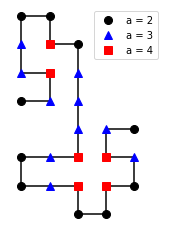
\includegraphics[width=0.24\textwidth, height=5cm]{Sections/Images/update.png}
    \caption{Пример конформации на квадратной решётке с подсчётом соседей}
    \label{fig:example_bulk}
\end{wrapfigure}


Сначала, чтобы определить правильность алгоритма расчёта долей искомых узлов, были проведены симуляции Монте-Карло модели ISAW при J=0 на длинах N от 5 до 3600, а так же произведены расчёты вручную для цепочек малых длин - от 5 до 11. Результаты изображены на рисунке \ref{fig:ISAW_Bulk_J0} - разные типы расчётов полностью совпали, что говорит о правильности использумоего алгоритма.

\begin{figure}[]
    \centering
    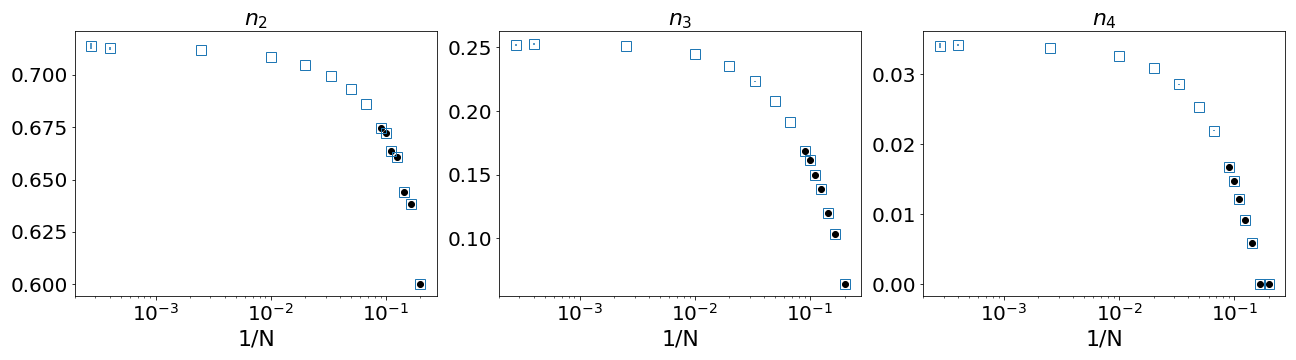
\includegraphics[width=0.95\textwidth]{Sections/Images/ISAWJ0_Bulk2-4.png}
    \caption{Зависимостей средних долей узлов конформации с фиксированным числом соседей (от 2 до 4) модели ISAW при J=0 от обратной длины 1/N при длинах конформации N=5-3600. Пустые квадраты - результаты симуляций Монте-Карло, черные точки - расчёты вручную}
    \label{fig:ISAW_Bulk_J0}
\end{figure}

\subsection{Особенности ранних результатов на квадратной решётке}

Мы провели симуляции Монте-Карло для долей узлов с фиксированным числом соседей для моделей Ising-ISAW и ISAW с зависимостью от значения константы взаимодействия J для длин N=1000, 2500, 3600, 4900. Результаты изображены на рисунке \ref{fig:Ising_vs_ISAW__2D_bulk}, а также опубликованы в статье Камиллы Файзуллиной \cite{faizullina2021critical}. 

\begin{figure}[h!]
    \centering
    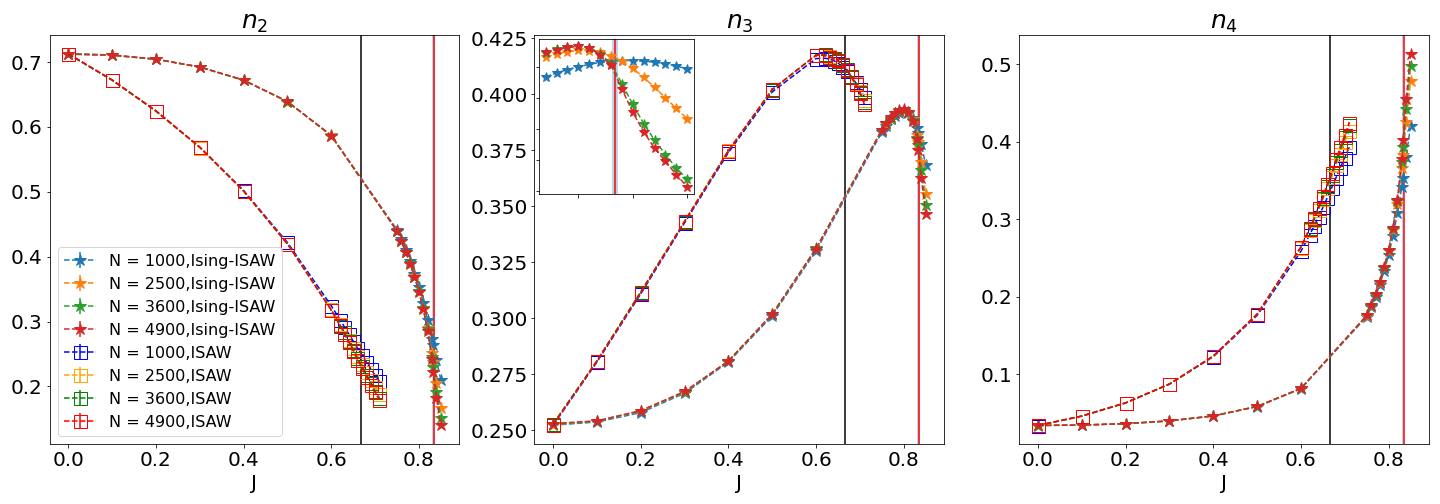
\includegraphics[width=0.95\textwidth]{Sections/Images/bulk2-4_inset.png}
    \caption{}
    \label{fig:Ising_vs_ISAW__2D_bulk}
\end{figure}

На графиках \ref{fig:Ising_vs_ISAW__2D_bulk} примечательны значения в точке J=0 у графиков узлов с 2-мя (левый) и 3-мя (средний) соседями: было первоначальное предположение, что в пределе бесконечной длины конформации они будут равны 3/4 и 1/4 соответственно. Так же интересен вопрос универсальности данного свойства на других решётках: будут ли эти соответсвующие значения долей при тех же условиях равны или хотя бы похожи в других решётках. 

\subsection{Сравнение модели Изинга и полимерной цепочки в решетках с 2-6 возможными соседями у мономеров}

Рассмотрим средние доли узлов с фиксированным числом соседей в решётках, которые имеют от 2-х до 6-ти возможных соседей: в кубической, у которой 5-й и 6-й соседи мономера расположены в соседний плоскостях, и треугольной, где 5-й и 6-й сосед мономера лежат на диагонали, проходящей через данный узел (в данной решётке лишь одна плоскость).

График зависимости долей от константы взаимодействия J изображен на рисунке \ref{fig:Ising_vs_ISAW} - слева показаны результаты симуляций Монте-Карло на кубической решётке, справа - на треугольной решётке. Цвета графиков соответствуют длинам цепочек - N=100 зелёные, 300 синие, 600 красные и 1200 фиолетовые. Число шагов симуляций - от $10^{10}$ вдали от пиков до $10^{12}$ в районе пиков графиков. Вертикальными линиями отмечены точки критического перехода: 

\begin{table}[h!]
    \centering
    \begin{tabular}{|c|c|c|}
        \hline
        lattice & Ising-ISAW & ISAW \\ \hline
        square & 0.8340(5)\cite{faizullina2021critical} &  0.6673(5)\cite{caracciolo2011geometrical} \\ \hline
        triangular & Unknown & 0.41(7) \cite{Privman1986}\\ \hline
        cubic & $0.5263 \pm 0.055$\cite{foster2021critical} & $0.2779 \pm 0.0041$\cite{Tesi1996} \\ \hline
    \end{tabular}
    \caption{Значения критических точек фазового перехода модели Изинга на случайном блуждании (Ising-ISAW) и гомополимера (ISAW) на квадратной, треугольной и кубической решётка соответственно (в порядке строк)}
    \label{tab:crits}
\end{table}

Результаты симуляций модели ISAW отмечены пустыми квадратами. Примечательно, что графики зависимости долей от J данной модели значительно плавнее, чем у модели Изинга на случайном блуждании, а так же процессы уплотнения конформаций (когда доли $n_{2}$ и $n_{3}$ уменьшаются, а доли узлов с большим числом соседей увеличивается) начинаются значительно раньше. В то же время, крайние пределы у данных моделей совпадают - графики одинанаковых длин и решёток разных моделей исходят из одной точки при J=0 (что логично, ведь при J=0 поведение Ising-ISAW соответствует ISAW) и приходят в одну точку при J=1.

Данные модели Ising-ISAW в свою очередь отмечены на графике \ref{fig:Ising_vs_ISAW} звездочками. Стоит отметить, что при прохождении точки перехода в кубической решётке, графики долей узлов с любым числов соседей словно претерпевают скачок, усиливающийся с ростом длины цепочки, в отличие от треугольной решётки, где процесс непрерывен.

Говоря о свойствах Ising-ISAW кубической решётки, необходимо подчеркнуть, что в на графике $\la n_{3} \ra$ мы видим похожее поведение в J=0 - значение довольно близко к 0.25, стоит проверить предел значения доли узлов с 3-мя соседями в J=0 при бесконечной длине и характер приближения к нему, если таковой имеется. Значение $\la n_{2} \ra$ при J=0 визуально отличается, но так же стоит проверить возможность предела.

\begin{figure}
    \centering
    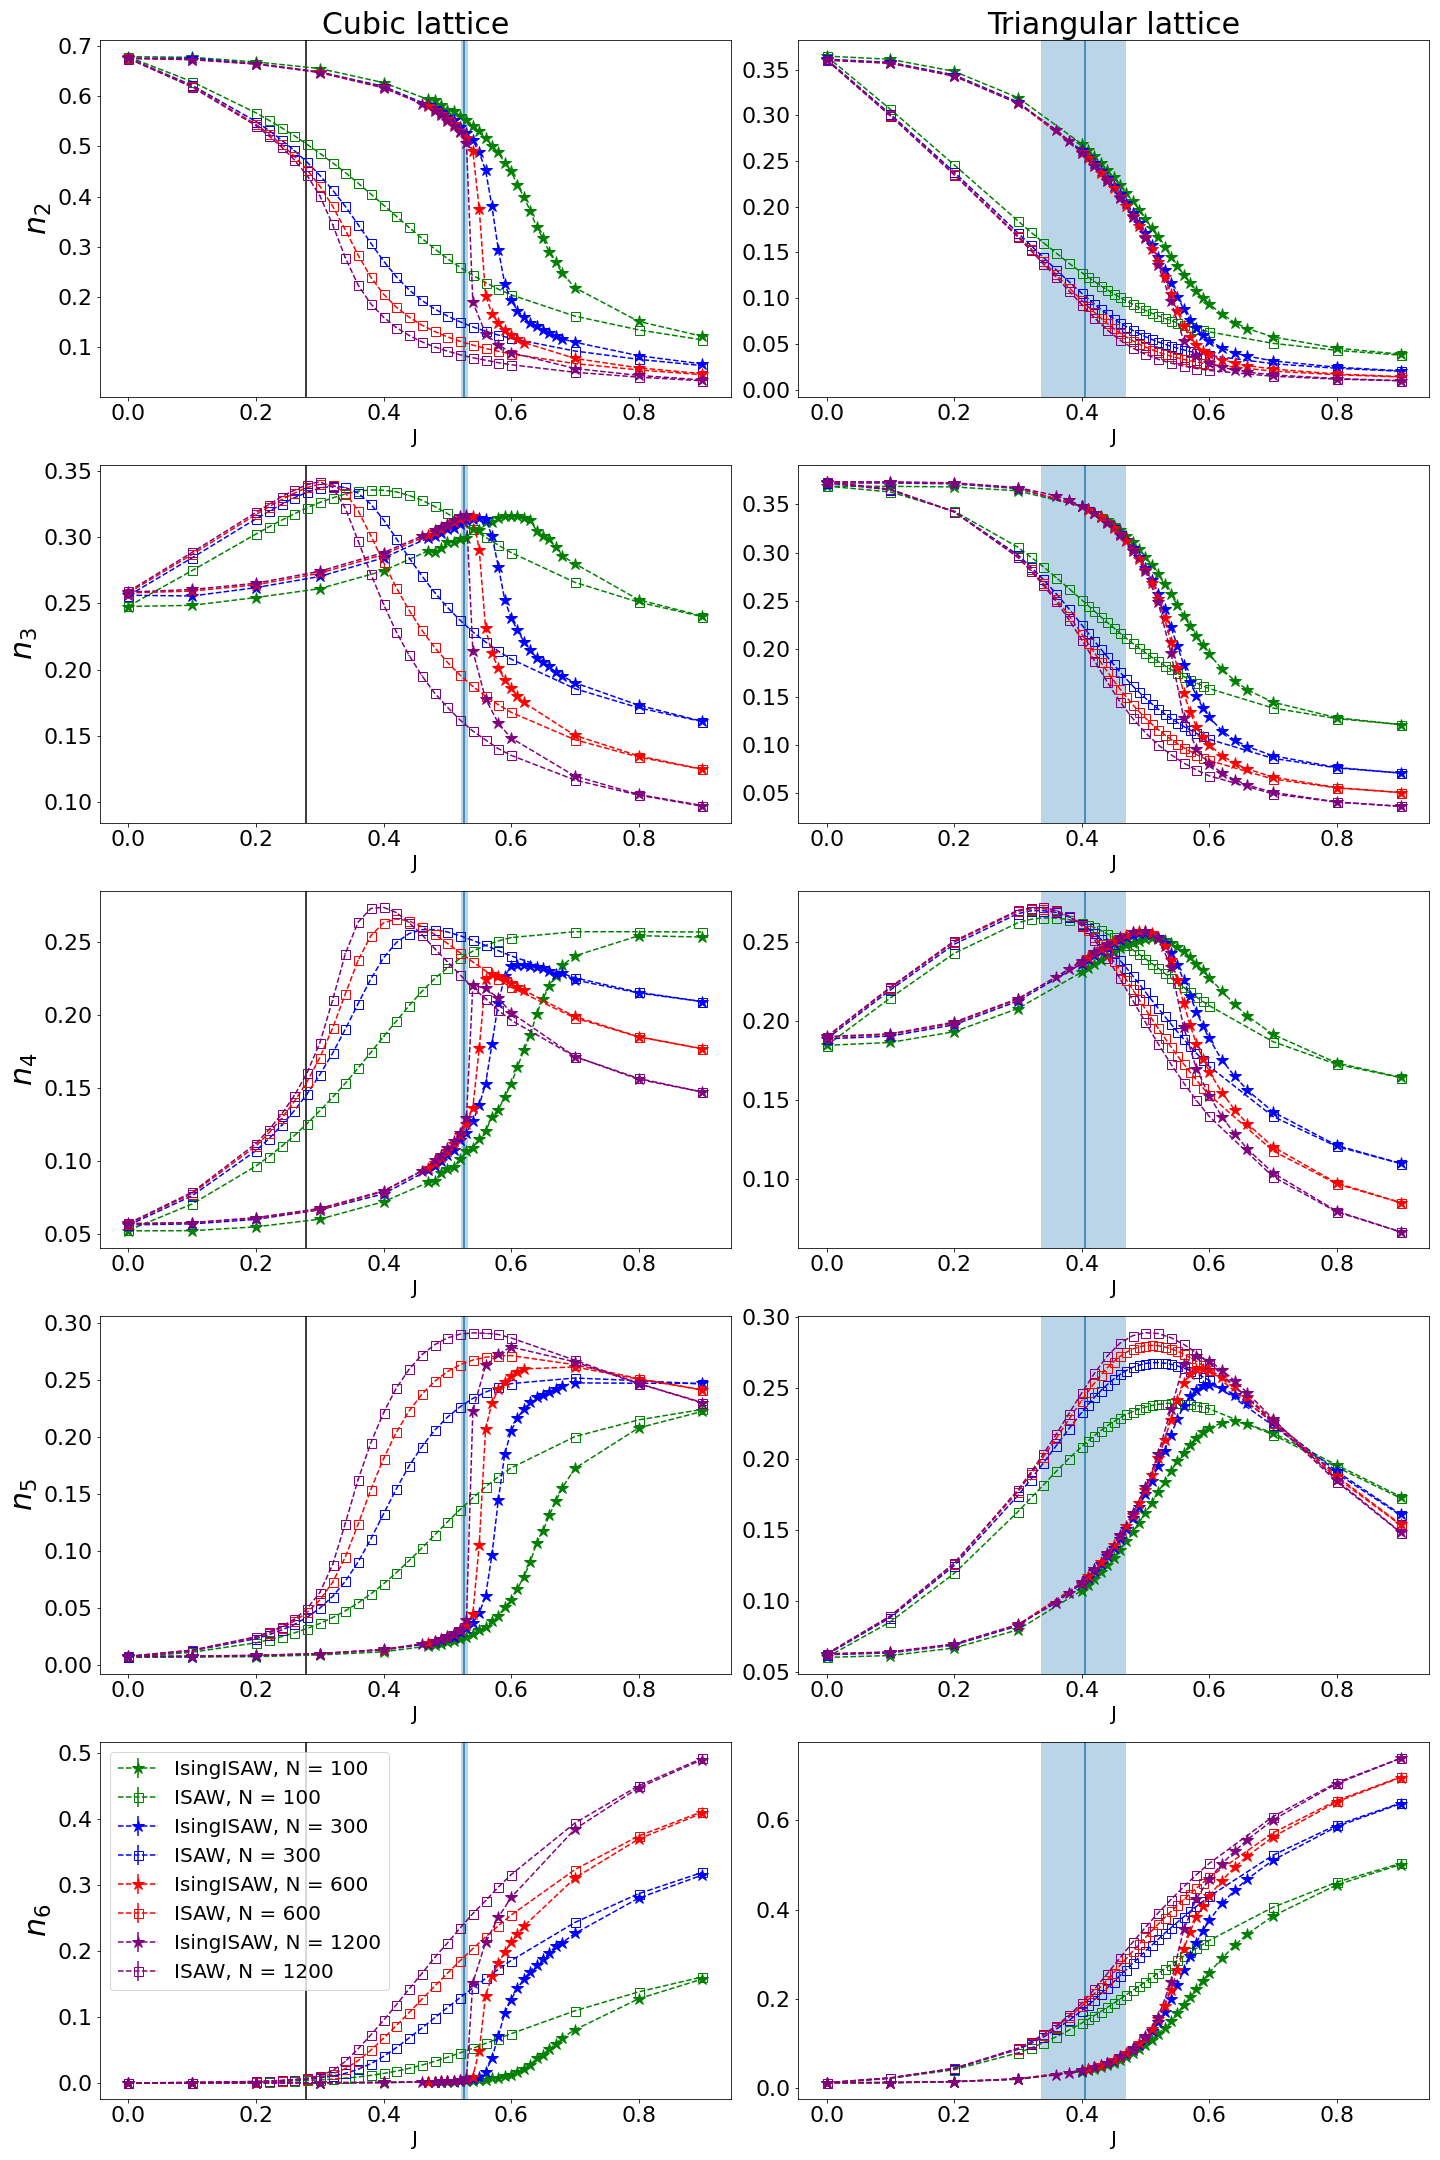
\includegraphics[width=0.95\textwidth, height=21.5cm]{Sections/Images/Ising_vs_ISAW.png}
    \caption{Fractions of monomers of Ising-ISAW model (stars) and ISAW model (open squares) on a cubic lattice (left column) and 2D-triangle lattice (right column) with 2-6 nearest neighbors as function of $J$ with length of conformations $N = $ 100 (green), 300 (blue) and 600 (red). Vertical lines define points of $\theta$-transition (For cubic lattice: black line for ISAW model \cite{Tesi1996} and blue line for Ising-ISAW model \cite{foster2021critical}; for triangle lattice: blue line for ISAW model \cite{Privman1986})}
    \label{fig:Ising_vs_ISAW}
\end{figure}

\newpage

\subsection{Алгоритм исследования характера зависимости значения долей узлов от длины при J=0}

Здесь рассматривается способ определения характера зависимости у графиков долей узлов с фиксированным числов соседей при J=0. Для примера взят случай $n_{2}$ у квадратной решётки модели Ising-ISAW. Первоначально рассматривается три возможных способа апроксимации результатов, варьирующихся зависимостью от обратной длины конформации $x = 1/N$:

\begin{enumerate}
    \item Линейная апроксимация $y = a x + b$
    \item Лог-линейная или экспоненциальная апроксимация $y = b \exp{(a x)} + c $
    \item Степенная или лог-лог апроксимация $y = b x^{a} + c  $
\end{enumerate}

Чтобы гарантировано получить результат использовалась функция linregress из пакета scipy.stats, поэтому на данном этапе погрешностью результатов симуляций мы временно пренебрегаем. Так же, чтобы показать нагляднее характер апроксимации, графики соответсвующих способов фитирования будут рассмотрены в том же масштабе - линейный в линейном, экспоненциальный в лог-линейном, степенном в лог-лог-масштабе - таким образом графики фитов будут линейными. Результаты апроксимаций в порядке, изложенном в списке выше, изображены на рисунках \ref{fig:square_scale_full} и \ref{fig:square_scale_limited} - в левом столбце апроксимации записаны для данных цепочек с длинами от 100 до 4900, в правом - длины от 250 до 4900, чтобы оценить поведение модели на больших длинах, следовательно, ближе к нулю.

\begin{figure}[h!]

\begin{minipage}{0.49\textwidth}
    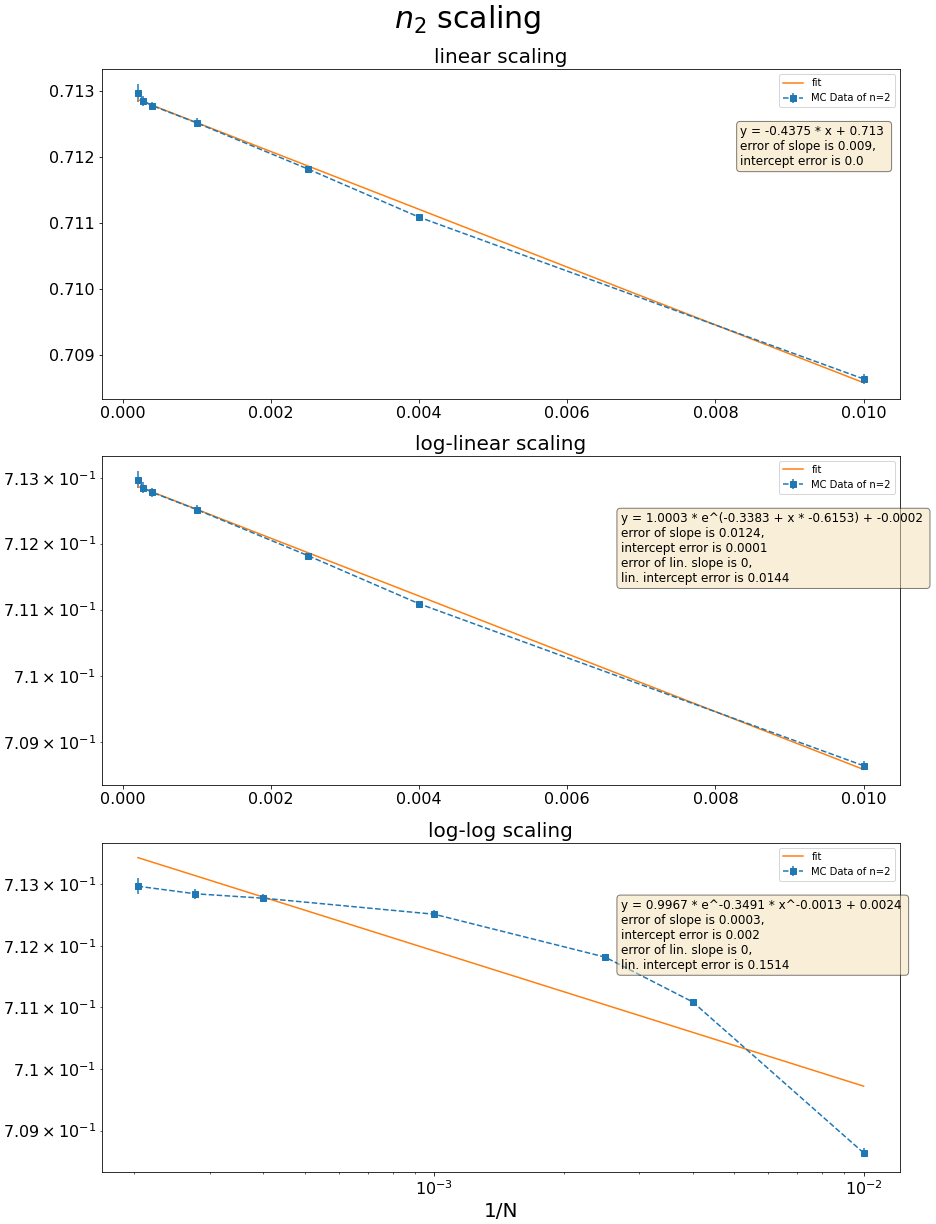
\includegraphics[width=\textwidth]{Sections/Images/square_n2_scaling.png}
    \caption{Результаты апроксимации (оранжевая линия) данных Монте-Карло о долей узлов с двумя соседями $n_2$ модели Ising-ISAW на квадратной решётке (синие точки) различными способами на диапазоне длин 100-4900}
    \label{fig:square_scale_full}
\end{minipage}
\hfill
\begin{minipage}{0.49\textwidth}
    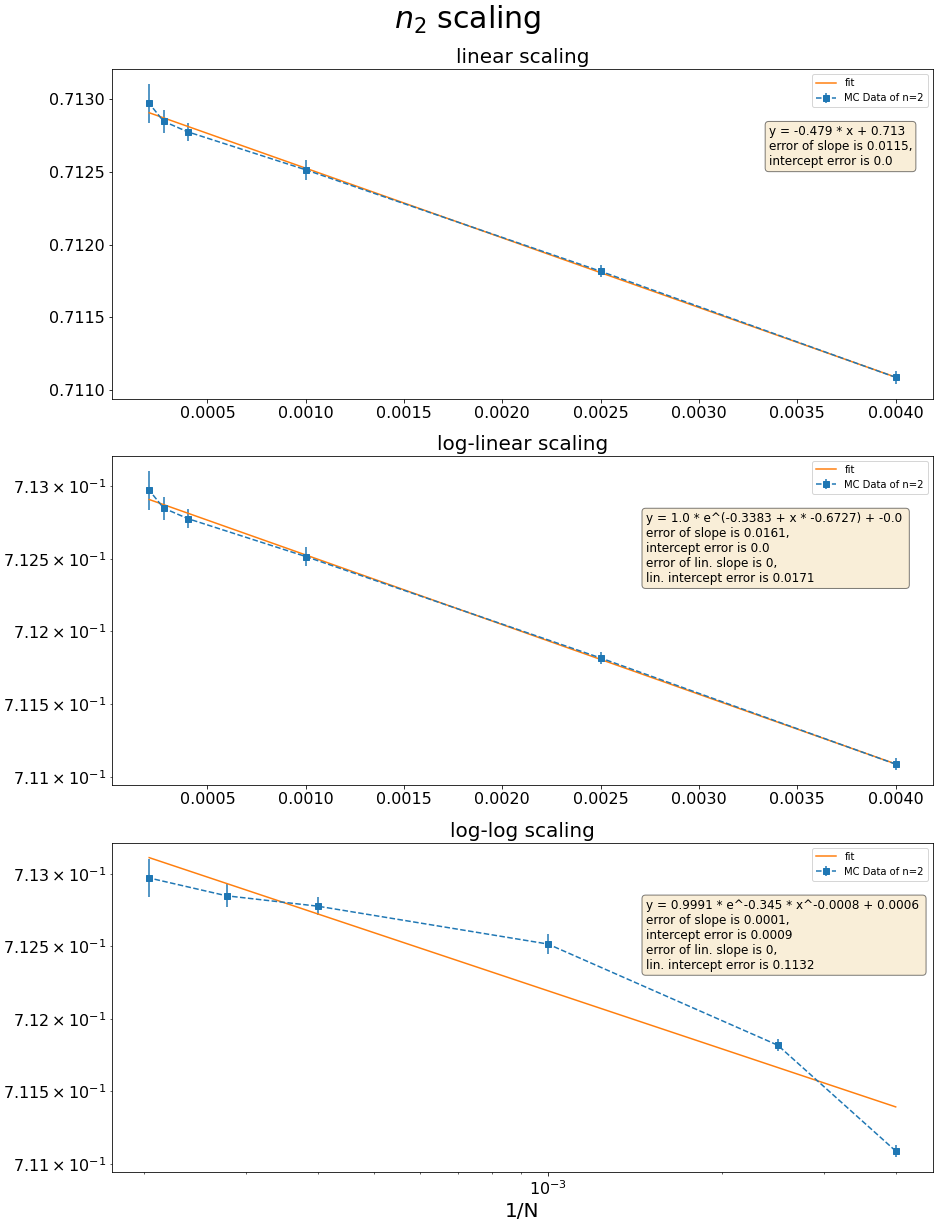
\includegraphics[width=\textwidth]{Sections/Images/square_n2_scaling2.png}
    \caption{Результаты апроксимации (оранжевая линия) данных Монте-Карло о долей узлов с двумя соседями $n_2$ модели Ising-ISAW на квадратной решётке (синие точки) различными способами на диапазоне длин 250-4900}
    \label{fig:square_scale_limited}
\end{minipage}
\end{figure}

Графики показывают, что в данном случае экспоненциальная апроксимация ведёт себя как линейная (что логично вблизи нуля), поэтому можно рассматривать вместо первых двух только линейную. С другой стороны, степенная функция совсем не совпадает с графиком результатов. Более того, значение степени функции-фита настолько мало, что итоговая функция больше похожа на константную прямую.

Таким образом, в данном случае определён линейный характер зависимости. Теперь, чтобы оценить качество приближения при рассмотрении точек всё ближе и ближе к нулю, оценим ошибку фитирования - теперь мы можем использовать функцию curve-fit из пакета scipy.optimize.

\begin{table}[]
    \centering
    \begin{tabular}{|c|c|c|} \hline
        N & a & b  \\ \hline
        100-4900 & -0.44(1) & 0.71292(4) \\ \hline
        250-4900 & -0.473(6) & 0.71299(2) \\ \hline
        400-4900 & -0.47(1) & 0.71298(2) \\ \hline
        1000-4900 & -0.48(6) & 0.71299(4) \\ \hline
    \end{tabular}
    \caption{Значения и погрешности коэффициентов линейного фитирования зависимости долей узлов с 2-мя соседями на квадратной решётке модели Ising-ISAW при J=0 от исследуемого интервала длин}
    \label{tab:a_b_n2_square}
\end{table}

Результаты показывают, что наиболее оптимальный фит достигается при выборе точек от 250 до 4900. Это можно объяснить тем, что при выборе точек большего диапазона линейный характер будет выражен слабее, а при выборе точек меньшего диапазона число данных уменьшается, что приводит к росту ошибки (недостаточно статистики). Подобная операция была выполнена и для других чисел соседей и решёток (см. Bulk2-6.ipynb в разделе "Расчёты ipynb" \cite{web:ProjectMagnetRepos}).

\subsection{Сравнение геометрических свойств модели Изинга на треугольной решётке с квадратной}

\begin{figure}
    \centering
    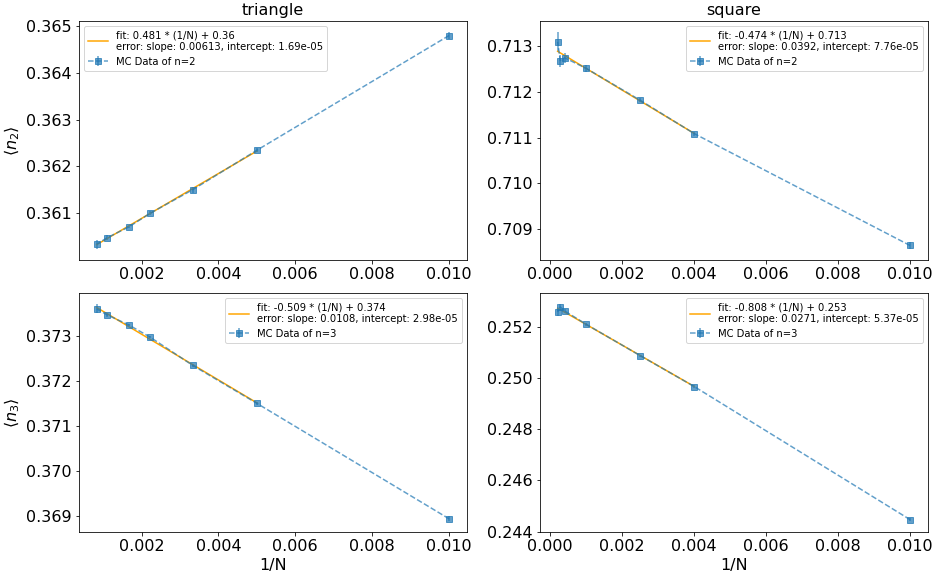
\includegraphics[width=0.95\textwidth]{Sections/Images/triagle_vs_square_bulk.png}
    \caption{Зависимость средней доли узлов с 2-3-мя соседями (сверху вниз) от обратной длины 1/N в модели Изинга на случайном блуждании на треугольной (справа) при N от 200 до 1200 и квадратной (слева) решётках при N от 250 до 4900 при J=0. Синяя линия описывает результаты симуляций Монте-Карло, оранжевая - график линейной апроксимации результатов, ошибки рассчитаны с учётом погрешностей полученных данных}
    \label{fig:tr_vs_sq_bulk}
\end{figure}

На графике \ref{fig:tr_vs_sq_bulk} наглядно показано сравнение приближений долей "одномерных" участков (то есть, долей мономеров с двумя соседями) и узлов с тремя соседями в цепочках на треугольной и квадратной решётках. Для расчётов долей на треугольной решётке были использованы длины 200-1200, для квадратной - 250-4900. Приближение долей треугольной решётки имеет отчётливый линейный характер, включая даже в приближении на всех точках (см. раздел "Подсчёт соседей у треугольной решётки" в Bulk2-6.ipynb \cite{web:ProjectMagnetRepos} ). Линейность долей квадратной решётки также подтверждается (с учётом погрешности расчётов с наибольшей длиной). 

\begin{table}[]
    \centering
    \begin{tabular}{|c|c|c|c|c|c|c|} \hline
        & \multicolumn{2}{|c|}{Square} & \multicolumn{2}{|c|}{Triangular} & \multicolumn{2}{|c|}{Cubic} \\ \hline
        Число соседей & a & b & a & b & a & b \\ \hline
        2 & -0.473(6) & 0.71299(2) & 0.491(3) & 0.35989(1) & 0.42(1) & 0.67429(3) \\ \hline
        3 & -0.809(4) & 0.25291(1) & -0.523(6) & 0.37411(1) & -1.270(7) & 0.26012(2) \\ \hline
    \end{tabular}
    \caption{Коэффициенты прямых, полученные линейным фитированием данных симуляций Монтекарло по долям соседей из рисунков \ref{fig:tr_vs_sq_bulk} и \ref{fig:tr_vs_cb_bulk}}
    \label{tab:fit_coeff}
\end{table}

Из таблицы \ref{tab:fit_coeff} по первым двум столбцам, отображабщим данные о прямых-фитов квадратной и треугольной решётки соответствено, сходства между одномерием треугольной и квадратной решётки с точки зрения самих приближений почти не наблюдается - они имеют как разные значения свободных членов, так и значения и даже (в случае 2-х соседей) знаки коэффициента наклона, разница который значительно превышает погрешность фита.



\subsection{Сравнение геометрических свойств модели Изинга на треугольной решётке с кубической}

\begin{figure}
    \centering
    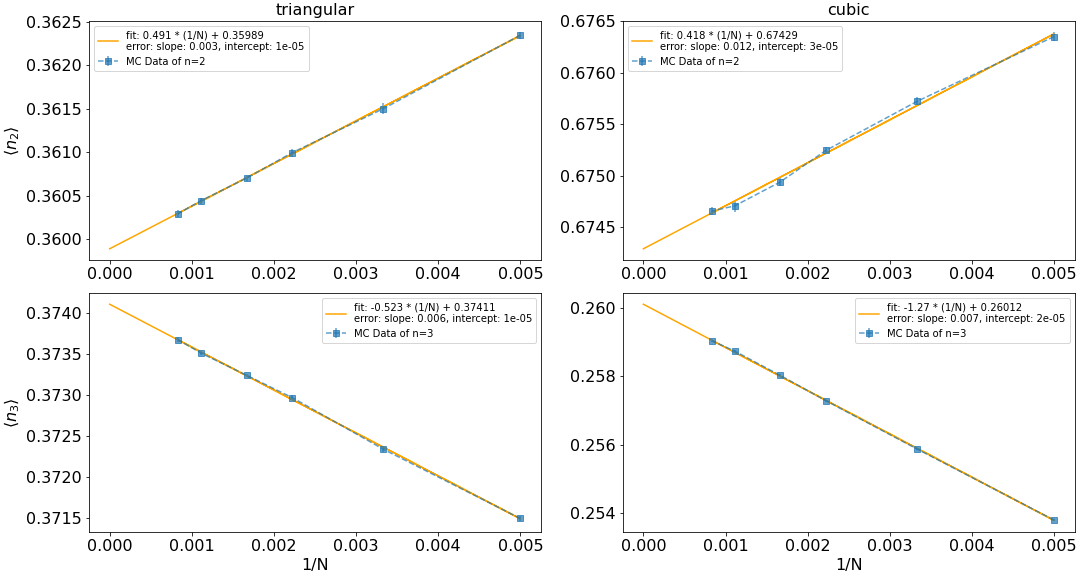
\includegraphics[width=0.95\textwidth]{Sections/Images/triangle_vs_cubic_bulk.png}
    \caption{Зависимость средней доли узлов с 2-3-мя соседями (сверху вниз) от обратной длины 1/N в модели Изинга на треугольной (слева) и кубической (справа) решётках при J=0. Синяя линия описывает результаты симуляций Монте-Карло, оранжевая - линейное приближение результатов, ошибки рассчитаны с учётом погрешностей полученных данных}
    \label{fig:tr_vs_cb_bulk}
\end{figure}

Здесь мы сравниваем линейное приближение треугольной решётки с кубической, имеющейтакое же количество возможных соседей. Рассматривая последние два больших столбца таблицы \ref{tab:fit_coeff}, где записаны коэффициенты прямых фитирования для $n_{2}$ и $n_{3}$ треугольной и кубической решётки соответственно, получается примерно та же ситуация как и в случае сравнения треугольной с квадратной - кубическая решётка на графике \ref{fig:tr_vs_cb_bulk} показывает почти чёткий линейный характер приближения в пределах погрешности наибольших длин (для n=3 линейно видна значительно лучше), но значения не имеют никакого сходства. Единственное отличие от сравнения с квадратной решёткой - графики соответствующих долей имеют одинаковое поведение с точки зрения знака наклона, что действительно и для долей узлов с больший числом соседей. Можно утверждать, что треугольная решётка с точки зрения поведения доли одномерных участок больше похожа на кубическую решётку, нежели квадратную, однако универсальность поведения доли "одномерных" участков среди решёток при бесконечно больших длинах конформации не обнаружена.

\subsection{Число соседей в атмосферах Преллберга}

Так же хочется заметить некоторое сходство значений свободного члена для долей с двумя соседями и свободного члена в приближениях графика зависимости вероятности гомополимерной цепочки иметь атмосферу 3 в статье Преллберга\cite{owczarek2008scaling}, то есть вероятность, что второй конец цепочки длины N имеет 3 возможных направления для удлинения и следовательно, 3 узла, которые могут стать N+1-ым в цепочке.

\begin{table}[]
    \centering
    \begin{tabular}{|c|c|c|c|}
    \hline
    k & $p^{(k)}$ & i & $intercept(\la n_{i} \ra)$ \\ \hline
    3 & 0.711 14(3) & 2 & $0.71299 \pm 2*10^{-5}$ \\ \hline
    2 & 0.225 00(2) & 3 & $0.25291 \pm 10^{-5}$ \\ \hline
    1 & 0.054 76(1) & 4 & $0.03410 \pm 10^{-5}$\\ \hline
    0 & 0.009 096(4) & - & - \\ \hline
    \end{tabular}
    \caption{Сравнение свободных членов линейных приближений вероятностей у конформации иметь n-ю атмосферу (слева) и долей мономеров с i соседями (справа) в зависимости от обратной длины конформации 1/N}
    \label{tab:Prellb_Compare}
\end{table}

На таблице \ref{tab:Prellb_Compare} слева изображены значения свободных членов графика зависимости вероятности гомополимерной цепочки иметь атмосферу k в статье Преллберга\cite{owczarek2008scaling}, то есть вероятность, что второй конец цепочки бесконечно большой длины N имеет k возможных направления для удлинения и следовательно, k возможных узлов, которые могут стать новым узлом в цепочке. Справа изображены значения свободных членов приближений графиков долей узлов с i соседями. Хотя все значения отличаются больше чем на погрешность расчётов, однако нельзя не заметить довольно близкое сходство $p^{(3)}$ и свободного члена $\la n_{2} \ra$, хотя сами приближения имеют противоположные по знаку наклоны. 
Возможно, обе величины по-разному описывают одно и то же поведение цепочек с точки зрения их плотности: например, если конец цепочки длины N (назовём его "N-ым узлом") имеет атмосферу три, то при добавлении нового N+1-го узла N-й будет иметь два соседа: N-1-й и N+1-й узлы. Так же при атмосфере 2 (то есть, уже имея два соседа и две возможности для удлинения) N-ый узел при удлинении будет иметь 3 соседа. И наконец, при атмосфере 1 удлинение цепочки приведёт к тому, что старый конец цепочки будет иметь 4 соседа. Очевидно, что случай удлинения при атмосфере 0 рассмореть невозможно, и провести аналогию с соседями нельзя.